\documentclass[aip,jcp,reprint]{revtex4-1}

\usepackage{natbib}

%\usepackage{libertine}
%\usepackage[libertine]{newtxmath}
%\usepackage{sansmath}
%\renewcommand{\familydefault}{\sfdefault}

\usepackage{color}
\usepackage{dcolumn}% Align table columns on decimal point
\usepackage{bm}% bold math
\usepackage{tabularx}
\usepackage{graphicx}
\usepackage{epstopdf}
\usepackage{mathtools}
\usepackage{amsmath}
\usepackage{eqnarray}

\newcommand{\un}[1]{\,\mathrm{#1}}  % for units
\newcommand{\bt}[1]{$\mathtt{#1}$}  % for beadtypes
\newcommand{\E}[1]{\cdot 10^{#1}}   % for normdarstellung

%%%%% BEGIN OF DOCUMENT %%%%%
%%%%%
\begin{document}


%%% TITLE, AUTHORS, AFFILIATION, ABSTRACT %%%
%%% 
\title{Local Structure Effects on Molecular Self-Diffusion}
\author{Jens Smiatek}
\email{smiatek@icp.uni-stuttgart.de}
\affiliation{Institute for Computational Physics, University of Stuttgart, Allmandring 3, D-70569 Stuttgart, Germany} 
\affiliation{Boehringer Ingelheim Pharm GmbH \& Co. KG, Development NCE, Birkendorfer Strasse 67, D-88397 Biberach (Riss), Germany} 
\author{Christian Holm}
\affiliation{Institute for Computational Physics, University of Stuttgart, Allmandring 3, D-70569 Stuttgart, Germany} 
\author{Samuel Tovey}
\affiliation{Institute for Computational Physics, University of Stuttgart, Allmandring 3, D-70569 Stuttgart, Germany} 

\begin{abstract}
We present the results of Langevin Dynamics (LD) simulations in combination with analytical calculations to describe the self-diffusion of tracer particles in continuum solvents. In terms of expressions for Fick and Maxwell-Stefan diffusion coefficients in binary solutions, we show that the self-diffusion coefficients exhibit a significant dependence on the local environment. According to Kirkwood-Buff theory, the respective self-diffusion coefficients depend on the derivatives of the thermodynamic activity, which changes significantly with the addition of further particles. These results show that the local environment has a decisive influence on the self-diffusion of particles. All simulation results show good agreement with the analytical expressions. The corresponding results thus provide a solid background for a deeper understanding of the relationships between local structures and their influence on the dynamics of individual particles.
\end{abstract}

\maketitle
%%%


%%% INTRO %%%
%%%

\section{Introduction}
Understanding diffusive motion is of fundamental importance for many technical applications. Almost all chemical separation processes such as distillation, absorption, extraction or condensation are based on the transport of substances within a liquid mixture or across a phase boundary \cite{seader06a,wankat22a}. The corresponding diffusion processes are often the rate-determining step for such separation mechanisms, which is why optimizing these processes also requires a fundamental understanding of diffusion. 
In general, one can distinguish between self-diffusion  and collective  or transport diffusion of  particles. 
In contrast to self-diffusion of isolated single particles,  transport diffusion can be regarded as a collective transport mechanism due to correlations between the components of a solution \cite{taylor93a,bird04a,newman12a,groot13a,liu13a,guevara16a,janzen17a}. 
In terms of their relevance for chemical and industrial processes, much effort has been spent on the investigation of diffusive behavior in different solvent mixtures \cite{maxwell67a,bird04a,newman12a, groot13a} in the form of numerical and experimental techniques \cite{kincaid83a,derlacki85a,vink85a,trullas93a,vergara01a, keffer05a,rehfeldt07a,krishna08a,krishna09a,rehfeldt10a,liu11a,moggridge12a,liu13a,parez13a,zhu15a,bardow15a,guevara16a,janzen17a}.\\
Whereas self-diffusion of tracer particles can be studied experimentally via advanced NMR measurements or microscopy techniques \cite{kashyap11a},  the investigation of transport diffusion by  Raman
spectroscopy, diaphragm cell techniques, interferometry,
microfluidics, or quasi-elastic neutron scattering experiments is far more complicated \cite{liu13a,taylor93a}. 
Moreover, the individual diffusion coefficients for components in binary mixtures  often reveal significant deviations from symmetric Maxwell-Stefan or Fick diffusion coefficients, such that the introduction of effective diffusion cefficients, even in non-porous environments, became obligatory \cite{taylor93a}.  In agreement with our limited knowledge in terms of multicomponent solutions, even the molecular mechanisms enforcing the occurrence of effective diffusion coefficients in binary mixtures are yet unknown \cite{taylor93a}. \\
Thus, most of previous works on diffusive motion rely on the evaluation of tracer diffusion which ignores the presence of other molecules  \cite{liu13a}.  However, these simplifications are often not really expedient, as molecular correlation processes often play an important role in the dynamics of liquids. A prominent example are correlations in electrolyte solutions  and their influence on the dynamic behavior and the resulting charge transport \cite{kashyap11a,smiatek18a}.
A crucial limitation for most charge transport processes is the formation of ion pairs  \cite{marcus06a,vanderVegt16a,smiatek18a,smiatek20a,narayanan18a,smiatek20b,miranda20a,yang20a,krishnamoorthy18b,smiatek19a}, whose occurrence significantly lowers the ionic conductivity as one of the most prominent examples \cite{schroder09a,krishnamoorthy16a,smiatek18a,smiatek20a,krishnamoorthy18c,nandy19a}. \\
Similarly, the role of local structures on diffusion processes is not yet fully understood in many cases. Especially in the last few years, some work linking the thermodynamic factors and the local environment within the framework of Kirkwood-Buff integrals has provided some new insights \cite{bardow15a,guevara16a,janzen17a,liu11a,liu13a,rosenberger20a}. Accordingly, it was shown that Maxwell-Stefan and Fick diffusion coefficients can be effectively calculated via consideration of the derivative of the thermodynamic activity \cite{bardow15a,guevara16a,janzen17a,liu11a,liu13a,rosenberger20a}. Thus, the previously hard to determine thermodynamic factors can be now written as simple expressions from Kirkwood-Buff theory \cite{kirkwood51,ben13a,pierce08a,smith06,smiatek17a,zingrebe18b,simon22a}. However, the corresponding simulations and expressions have so far only been evaluated for collective diffusion, whereby self-diffusion has not yet been taken into account. Interestingly,  molecular self-diffusion is of great interest for some processes such as diffusion in nanopores or in confined geometry as well as for crowded solutions, so that the influence of the local environment by means of the description of expressions of Kirkwood-Buff theory would also provide interesting insights \cite{simon22a,jamali18a,jamali20a,roosen11a,dix08a}.
In this article, we present expressions for self-diffusion coefficients of tracer particles with increasing concentration. We show that the local environmental structure in terms of Kirkwood-Buff integrals as well as the corresponding derivative of the thermodynamic activity crucially influences the diffusive behavior.  Our mathematical expressions are validated by Langevin Dynamics (LD) simulations which allow us a detailed comparison with the analytical findings. \\
The paper is organized as follows. In the next section, we present the theoretical background of our approach in combination with the corresponding new expression. In the third section, we discuss  the details of the 
simulations. All computational results are  presented in the fourth section. 
We conclude with a summary in the last section.

\section{Theoretical Background}
As a standard approach for  the description  of correlated diffusive motion of molecules in a mixture, the molar flux $J_{\alpha}$ of component $\alpha$ in a solution with $C$ components can be written by the generalized Fick law \cite{liu13a,bird04a}
\begin{equation}
\label{eq:fick1}
J_{\alpha}=- \rho \sum_{\beta=1}^{C-1} D_{\alpha\beta} \nabla x_{\beta}
\end{equation}
with the total bulk number density $\rho=\sum_{\alpha=1}^CN_{\alpha}/V$, including $N_{\alpha}$ molecules of species $\alpha$ in volume $V$. As can be seen, the mass flux $J_{\alpha}$ depends on the gradient of the the mole fraction $x_{\alpha}=\rho_{\alpha}/\rho$ and is proportional to the Fick or transport diffusion coefficients $D_{\alpha\beta}$ with $\beta=1,\ldots,C-1$. 
For binary mixtures $(C=2)$ with components $\alpha\neq \beta$ and with regard to momentum conservation in terms of  $J_{\alpha} = - J_{\beta}$,  it follows that only a single Fick diffusion coefficient $D=D_{\alpha\beta}=D_{\beta\alpha}$ for both components exists \cite{liu13a,taylor93a,newman12a}. This Fick diffusion coefficient can be combiend with Eqn.~\eqref{eq:fick1} in terms of 
\begin{equation}
\label{eq:fickbin}
J_{\alpha}= -\rho D \nabla x_{\alpha}.
\end{equation}
due to reasons of symmetry.\\
In addition to the Fick law, a further expression for diffusion in multicomponent mixtures \cite{liu13a} is  represented by the 
Maxwell-Stefan relation \cite{liu13a,bird04a}
\begin{equation}
\label{eq:msd}
\frac{1}{RT}\nabla\mu_{\alpha} = -\sum_{\alpha=1,\alpha\neq \beta}^{C}\frac{(\mathbf{v}_{\alpha}-\mathbf{v}_{\beta})}{D_{\alpha\beta}^{\text{MS}}}x_{\beta}
\end{equation}
where $R$ and $T$ denote the universal gas constant and absolute temperature, respectively, with the chemical potential $\mu_{\alpha}$ of species $\alpha$, the average velocity vectors $\mathbf{v}_{\alpha}$ and $\mathbf{v}_{\beta}$ of the corresponding species and the Maxwell-Stefan diffusion coefficients $D_{\alpha\beta}^{\text{MS}}$.
In more detail, the Maxwell-Stefan diffusion coefficient can be interpreted as a tensor of  inverse friction coefficients between distinct  components of the solution. In contrast to Fick diffusion coefficients, Maxwell-Stefan diffusion coefficients do not depend on a reference frame, are  less prone to concentration variations, include non-ideal solution effects, and  are symmetric with $D_{\alpha\beta}^{\text{MS}}=D_{\beta\alpha}^{\text{MS}}$ for multicomponent solutions with $C\geq 2$.\\ Noteworthy, for low densities of a single component $\alpha$  in binary mixtures, the Maxwell-Stefan, Fick and self-diffusion or tracer diffusion coefficients become identical  in accordance with the relation\cite{liu13a}  $\lim_{\rho_{\alpha}\rightarrow 0}D_{\alpha\beta}=\lim_{\rho_{\alpha}\rightarrow 0}D_{\alpha\beta}^{\text{MS}} = \lim_{\rho_{\alpha}\rightarrow 0} D_{\alpha\alpha}^s$  with self-diffusion coefficient $D_{\alpha\alpha}^s$ \cite{bardow15a,,liu11a,liu13a}.
Furthermore, a linear relation between the Maxwell-Stefan- and the Fick diffusion coefficients can be defined, which reads 
\begin{equation}
\label{eq:msdiffusion}
D= D^{\text{MS}}\cdot \Gamma,
\end{equation}
for a binary solution \cite{taylor93a,balsara15a,janzen17a}  including  the symmetric thermodynamic factor\cite{guevara16a,janzen17a,lecce17a}
\begin{equation}
\label{eq:thermodyn_fact}
\Gamma=\frac{x_{\alpha}}{RT}\left(\frac{\partial \mu_{\alpha}}{\partial x_{\alpha}}\right)_{T,p}
\end{equation}
at constant temperature $T$ and pressure $p$.\\
In terms of a more detailed interpretation, thermodynamic factors account for the non-ideality of the solution, and thus provide a connection between transport mechanisms and thermodynamics.  Notably, non-ideal effects are  evident for all values $\Gamma \neq 1$ as for most real solutions, which highlights their potential importance for diffusive processes with regard to Eqn.~\eqref{eq:msdiffusion}.\\
In accordance with the relation
\begin{equation}
\label{eq:Gamma}
\frac{x_{\alpha}}{RT}\left(\frac{\partial \mu_{\alpha}}{\partial x_{\alpha}}\right)_{T,p} = \frac{1}{RT}\left(\frac{\partial \mu_{\alpha}}{\partial \ln \rho_{\alpha}}\right)_{T,p},
\end{equation}
one can insert the basic definition of the chemical potential
\begin{equation}
\mu_{\alpha} = \mu_{\alpha}^0 + RT\ln a_{\alpha}
\end{equation}
with the thermodynamic activity $a_{\alpha}$ into Eqn.~\eqref{eq:Gamma}, leading to
\begin{equation}
\label{eq:KBGamma}
\frac{1}{RT}\left(\frac{\partial \mu_{\alpha}}{\partial \ln \rho_{\alpha}}\right)_{T,p}=\left(\frac{\partial \ln a_{\alpha}}{\partial \ln \rho_{\alpha}}\right)_{T,p}
\end{equation}
with the derivative of the  thermodynamic activity  $a_{\alpha\alpha} = \left(\partial \ln a_{\alpha}/\partial \ln \rho_{\alpha}\right)_{T,p}$. For a binary solution, this expression can also be written in the framework of Kirkwood-Buff theory \cite{ben13a,smiatek18a,pierce08a,smith06}
according to 
\begin{equation}
\label{eq:act}
a_{\alpha\alpha} = \left(\frac{\partial \ln a_{\alpha}}{\partial \ln \rho_{\alpha}}\right)_{T,p} = \frac{1}{1+\rho_{\alpha}(G_{\alpha\alpha}-G_{\alpha\beta})}
\end{equation}
with the Kirkwood-Buff integrals 
\begin{equation}
\label{eq:KBI}
G_{\alpha\beta} = 4\pi \int_0^{\infty}r^2\, (g_{\alpha\beta}(r) - 1)\,\textrm{d}r
\end{equation}
including the radial distribution function $g_{\alpha\beta}(r)$ between two species $\alpha$ and $\beta$. In consequence, the thermodynamic factor $\Gamma$ can be identified as the derivative of the thermodynamic activity $\Gamma_{\alpha} = a_{\alpha\alpha}$, such that Eqn.~\eqref{eq:msdiffusion} reads 
\begin{equation}
\label{eq:DMS}
D= D^{\text{MS}}\cdot a_{\alpha\alpha} =  D^{\text{MS}}\cdot \left( \frac{1}{1+\rho_{\alpha}(G_{\alpha\alpha}-G_{\alpha\beta})}\right)
\end{equation}
which already highlights the integral importance of the local environment on the diffusion process in terms of the Kirkwood-Buff integrals. \\
For a binary solution, it was shown that the Maxwell-Stefan diffusion coefficients can be written as \cite{liu13a,rosenberger20a}
\begin{equation}
\label{eq:comp}
D^{\text{MS}} = \frac{x_2}{x_1}D_{11} + \frac{x_1}{x_2}D_{22} - 2D_{12}
\end{equation}
with the Onsager diffusion coefficients $D_{ij}$. 
The Onsager diffuson coefficients can also be written as \cite{liu13a}
\begin{equation}
D_{ij}= \frac{1}{3N}\int_0^{\infty}\textrm{d}t^{\prime}\left \langle \sum_{l=1}^{N_{\alpha}}\mathbf{v}_{l,i}(t)\cdot \sum_{m=1}^{N_{\beta}}\mathbf{v}_{m,j}(t+t^{\prime})\right\rangle
\end{equation}
with the velocities $\mathbf{v}$ of $N_{\alpha}$ and $N_{\beta}$ species, respectively for different sorts of molecules at different time points.
Moreover, it can be seen that the first Onsager coefficient $D_{11}$  can be decomposed into self-diffusion and cross-diffusion coefficients according to $D_{11} = D_{11}^s + D_{11}^c$ with
\begin{equation}
D_{11}^s= \frac{1}{3N}\int_0^{\infty}\textrm{d}t^{\prime}\left \langle \sum_{l=1}^{N_{\alpha}}\mathbf{v}_{l,1}(t)\cdot \mathbf{v}_{l,1}(t+t^{\prime})\right\rangle
\end{equation}
and 
\begin{equation}
D_{11}^c= \frac{1}{3N}\int_0^{\infty}\textrm{d}t^{\prime}\left \langle \sum_{l=1}^{N_{\alpha}}\mathbf{v}_{l,1}(t)\cdot \sum_{m\neq l}^{N_{\alpha}}\mathbf{v}_{m,1}(t+t^{\prime})\right\rangle.
\end{equation}
Insertion of these relations into Eqn.~\eqref{eq:comp} and Eqn.~\eqref{eq:msdiffusion} gives
\begin{equation}
D= \left(\frac{x_2}{x_1}(D_{11}^s+D_{11}^c) + \frac{x_1}{x_2}D_{22} - 2D_{12}\right)\cdot a_{11} 
\end{equation} 
which finally yields 
\begin{equation}
\label{eq:tracer}
D_{11}^s = \frac{x_1}{x_2}\left(\left(\frac{D}{a_{11}}\right)+2D_{12}\right)-\frac{x_1^2}{x_2^2}D_{22}-D_{11}^c
\end{equation}
for the self-diffusion of tracer particles in binary systems.\\
If we assume Brownian particles at low density in combination with a continuum solvent approach, meaning that the solvent molecules are continuous and thus not correlated, Eqn.~\eqref{eq:comp} reduces to
\begin{equation}
D = D_{11}^s+D_{11}^c \approx D_{11}^s,
\end{equation}
which violates the law of mass conservation in the generalized Fick law (Eqn.~\eqref{eq:fickbin}). In consequence, the relation
\begin{equation}
\label{eq:tracerdiff}
D_{11}^s = \left(\frac{D}{a_{11}}\right) - D_{cm}
\end{equation}
has to be extended by a center-of-mass difusion coefficient $D_{cm}$  in order to correct for these contributions with regard to $J_1 = - J_2$. \\
Hence, the combination of Eqn.~\eqref{eq:tracerdiff}  with Eqn.~\eqref{eq:act} according to
\begin{equation}
D_{11}^s = D(1+\rho_1(G_{11}-G_{12})) - D_{cm}
\end{equation}
already shows that the local environment in terms of further tracer particles influences the self-diffusion processes of the individual particles.  \\
Comparable conclusions can also be drawn with regard to the Darken relation \cite{rosenberger20a,liu11a,liu13a,darken48a} according to 
\begin{equation}
D^{\text{MS}} \approx x_2 D_{11}^c + x_1 D_{22}^c
\end{equation}
which also leads to a simplification of Eqn.~\eqref{eq:DMS}. 

\section{Simulation Details}
We performed  Langevin Dynamics (LD) simulations for a varying amount of single particles in a continuum solvent. The systems were simulated with  the GROMACS 5.0.2 software package \cite{vanderspoel05a,gromacs08a,pronk13a}.
The spherical particles were modified from  the GROMOS 43a1 force field \cite{gunsteren96a}. The corresponding mass of the particles was set identical to sodium ions Na$^+$ (atomtype 'NA') while the Lennard-Jones interaction parameters were taken from Zn$^{2+}$ ions (atom type 'ZN2+'). In addition, the charge was set to zero. The smaller mass of sodium was chosen to achieve an efficient sampling of the phase space for the given time scale. In addition, slight attractive dispersion interactions as represented by the Lennard-Jones parameters from the Zn$^{2+}$ ions enforce weak particle interactions and accumulation. 
Moreover, we also simulated individual SPC water molecules \cite{berendsen81a} in a homogeneous continuum solvent with the same approach as for the spherical particles to test the influence of non-spherical objects. It should be noted that the expressions from the Kirkwood-Buff theory do not depend on the shape of the particles \cite{ben13a,smiatek17a,smith06,pierce08a}, such that the corresponding expression for the self-diffusion coefficient (Eqn.~\eqref{eq:tracer} are universally applicable.
Further that the corresponding force field parameters still correspond to molecular time and length scales, so that the assumption of a random motion of these particles in an implicit solvent seems questionable. However, it is not our aim to reproduce any kind of experimental behaviour for which new force fields might have to be parameterized, which would go beyond the scope of this work. Accordingly, our results are also applicable to larger length and time scales where stochastic motion becomes relevant.\\
A leap-frog stochastic dynamics integrator \cite{vangunsteren88a} was used to reproduce the stochastic motion of the particles. The equation of motion reads 
\begin{equation}
\label{eq:LD}
m_i\dot{\textbf{v}}_i(t) = {\textbf{F}}_i^R(t)-m_i\gamma_i{\textbf{v}}_i(t)+{\textbf{R}}_i(t)
\end{equation}
with the mass $m_i$ of a particle $i$ fom the chosen species, the velocity $\textbf{v}_i$, the conservative forces $ {\textbf{F}}_i^R(t)$, the friction coefficient $\gamma_i$ and the random force ${\textbf{R}}_i$. The random force obeys the conditions of Gaussian white noise in terms of 
\begin{equation}
\langle R_{\alpha,i}(t)R_{\beta,j}(t_0)\rangle = 2 m_i k_BT \delta_{ij}\delta_{\alpha\beta}\delta(t-t_0)
\end{equation}
in combination with  $\langle {\textbf{R}}_i(t)\rangle = 0 $. The temperature was set to $T=300$ K in all runs and the friction coefficient was chosen as $\gamma = 0.5$ ps$^{-1}$. 
We used NVT simulation with a fixed length of $L_B = 3$ nm for the cubic simulation boxes. Constant box lengths are essential to avoid varying finite size effects for our calculations \cite{yeh04a}. Random insertion of $N=20, 22, 24, 26, 28, 30, 32,34,36, 38, 40, 42$ and $44$ spherical particles for the individual  simulations resulted in different number densities ranging from $\rho_1 =  (0.78 - 1.71)$ nm$^{-3}$. The corresponding water particle simulations correspond to $N = 2,3,4,5$ and 6 water molecules resulting in particle densities of $\rho_1 = (0.08 - 0.23)$ nm$^{-3}$. Each system was simulated for 50 ns with a time step of $\Delta$t = 2 fs and the first 2 ns were used for equilibration. 


\section{Results}
In the following, we denote all solute particles with the subscript "1", while the continuum phantom solvent is denoted with the subscript '2'.
\subsection{Spherical Particles}
The radial distribution functions $g_{11}(r)$ for chosen particle densities  are presented in Fig.~\ref{fig1}. 
\begin{figure}[tbh!]
        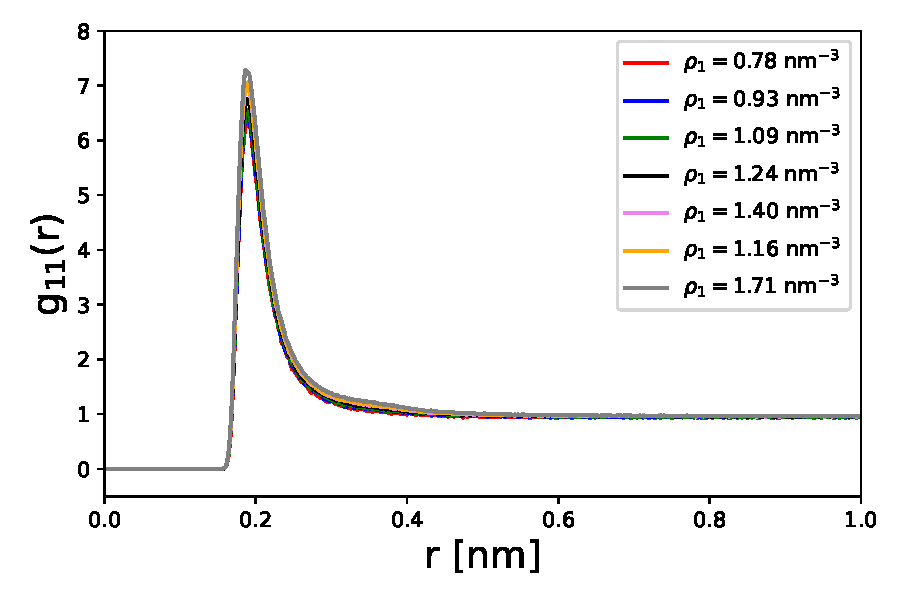
\includegraphics[width=0.5\textwidth]{fig1.pdf} \\
        \caption{Center-of-mass radial distribution functions $g_{11}(r)$ for different densities of spherical particles.}
        \label{fig1}
\end{figure}
As can be seen, the particles reveal a pronounced short-range ordering as reflected by the high peak values at $r \approx 0.19$ nm. This local  ordering can be attributed to the attractive part of the Lennard-Jones potential which induces slight accumulation effects in terms of first contact shells. In accordance, one can recognize a steep decrease of  the radial distribution functions with a convergence to $g_{11}(r)\approx 1$ at distances $r\geq 0.8$ nm which highights the transition from local to  bulk regions. At particle densities of $\rho_1 \geq 1.40$ nm$^{-3}$, a slight shoulder formation between $r= (0.25 - 0.5)$ nm can be seen, which indicates the formation of larger or even second-order contact pair shells. In summary, one can conclude that the particles show slight accumulation effects due to attractive Lennard-Jones potentials.\\
These effects become also evident in terms of the potential of mean forces \cite{chandler87a} according to 
\begin{equation}
\label{eq:pmf}
\mathrm{PMF}(r) = - k_BT\ln g_{11}(r)
\end{equation}
as shown in Fig.~\ref{fig2}. 
\begin{figure}
        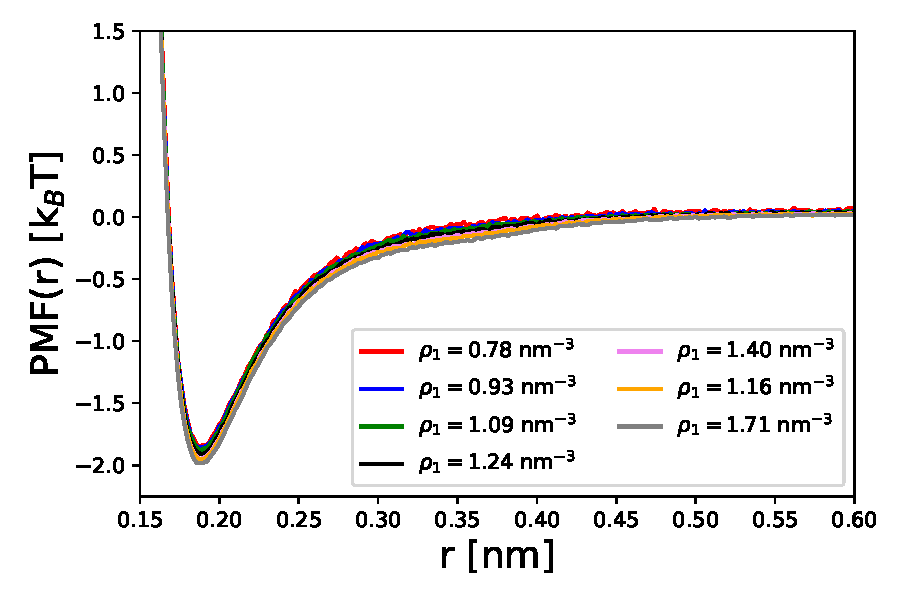
\includegraphics[width=0.5\textwidth]{fig2.pdf} \\
        \caption{Potential of mean forces calculated from Eqn.~\eqref{eq:pmf} for different densities of spherical particles.}
        \label{fig2}
\end{figure}
Despite the large variation in particle densities, it becomes obvious that the potential of mean forces is largely comparable, with differences in the maximum values around $\Delta$PMF $\approx 0.2 k_BT$.  Moreover, it can be seen that these forces are attractive on length scales up to 0.55 nm with a maximum value of PMF $\approx -(1.8 - 2.0) k_BT$ at $r= 0.19$ nm.  The corresponding findings highlight that accumulation is driven by attractive interactions whose values allow for a proper binding and unbinding equilibrium. According to the rather low energy barriers, the particles are free to move in the simulation box with a moderate tendency for accumulation. \\
Such findings are also evident with regard to the running Kirkwood-Buff integrals $G_{11}(r)$ (Eqn.~\eqref{eq:KBI} as shown in Fig.~\ref{fig3}. 
\begin{figure}
        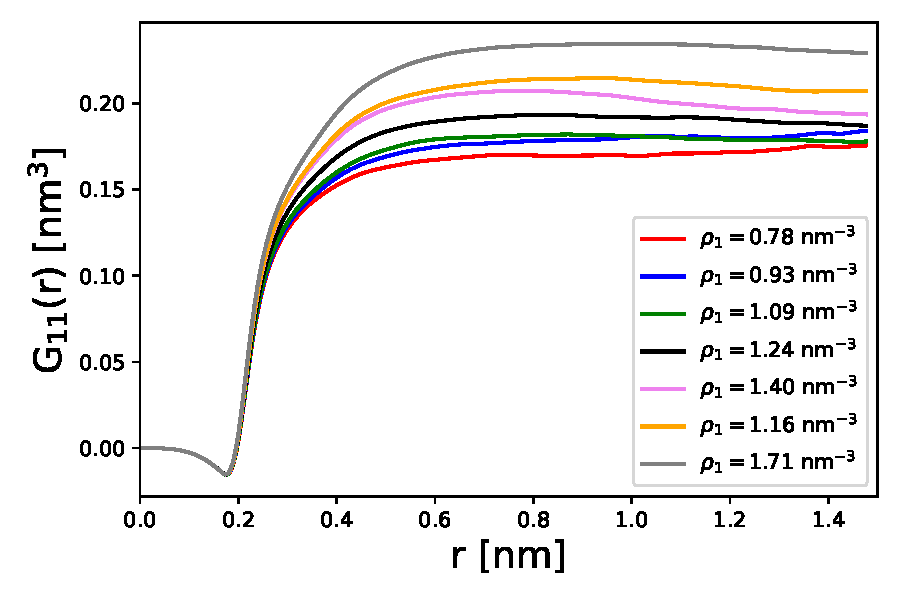
\includegraphics[width=0.5\textwidth]{fig3.pdf} \\
        \caption{Running Kirkwood-Buff integrals $G_{11}(r)$ for different densities of spherical particles.}
        \label{fig3}
\end{figure}
In general, Kirkwood-Buff integrals can be interpreted as excess volumes relative to the ideal state \cite{smiatek17a}. 
Accordingly, all Kirkwood-Buff integrals for particles with finite size and fixed diameter show a slight decrease at short distances, which is interpreted as an excluded volume effect. This is also evident for distances $r < 0.19$ nm. A rapid increase of the Kirkwood-Buff integrals can be observed between $r = (0.20 - 0.30)$ nm which corresponds to the first contact pair shell in agreement with Fig.~\ref{fig1}. For larger distances than $r \geq 0.8$ nm, the Kirkwood-Buff integrals finally converge to a constant value as defined by Eqn.~\eqref{eq:KBI}. With reference to Fig.~\ref{fig3}, the corresponding values of $G_{11}$ are ordered as a function of particle density. This means that higher particle densities lead to larger Kirkwood-Buff integrals. Such findings are consistent with the accumulation effects already observed. Since Kirkwood-Buff integrals represent the deviation from an ideal state, it can be concluded that higher particle densities deviate more strongly from a homogeneous distribution. \\ 
Comparable findings can also be observed for the preferential binding coefficients $\nu_{11}(r)$ and the derivatives of the thermodynamic activity $a_{11}(r)$ as shown in Fig.~\ref{fig4}. 
The preferential binding coefficient, defined by \cite{smiatek17a,zingrebe18b}
\begin{equation}
\label{eq:nu11}
\nu_{11}(r) = \rho_1(G_{11}(r)-G_{12}(r))
\end{equation}
allows us to estimate the tendency of the aggregation effects. For positive values we can identify a preferential binding mechanism and for negative values a preferential exclusion effect \cite{smiatek17a,zingrebe18b,smiatek18a}.  As can be seen, the second Kirkwood-Buff integral $G_{12}(r)$ denotes the interaction between the particles and the implicit continuum solvent. In general, implicit solvents lead to radial distribution functions $g_{12}(r) = 1$, so that $G_{12}(r) = 0$ (Eqn.~\eqref{eq:KBI}) and thus to the approximation 
\begin{equation}
\nu_{11}(r) = \rho_1 G_{11}(r) 
\end{equation}
whose values are shown in the upper panel of Fig.~\ref{fig4}. As can be seen, the converged values for distances larger than $r = 0.6$ nm are positive and show nearly comparable differences for densities $\rho_1 = (0.78 - 1.16)$ nm$^{-3}$. Accordingly, one can assume that the strength of the preferential binding mechanism increases monotoneously with increasing particles densities. However, a slight change can be observed for higher particle densities such that the preferential binding coefficients for particle densities  $\rho_1 \geq 1.24$ nm$^{-3}$ and  $\rho_1 \geq 1.16$ nm$^{-3}$ are nearly comparable. In accordance with Fig.~\ref{fig1}, one can attribute these findings to the formation of the second contact pair shell. These rather non-linear contributions also lead to differences in the preferential binding coefficients as can be seen for particle densities $\rho_1 \geq 1.46$ nm$^{-3}$. The largest  preferential binding coefficient can be observed for the highest particle density which also reveals the strongest accumulation effect.\\
In accordance with Eqn.~\eqref{eq:nu11}, the derivative of the thermodynamic activity  (Eqn.~\eqref{eq:act}), can also be written as 
\begin{equation}
a_{11} = \left(\frac{\partial \ln a_1}{\partial \ln \rho_1}\right)_{T,p} = \frac{1}{1+\nu_{11}}
\end{equation}
which highlights the pronounced influence of the local structure in terms of accumulation effects for the thermodynamic activity. The corresponding results for the derivatives of the thermodynamic activity are shown in the lower panel of Fig.~\ref{fig4}. 
\begin{figure}
        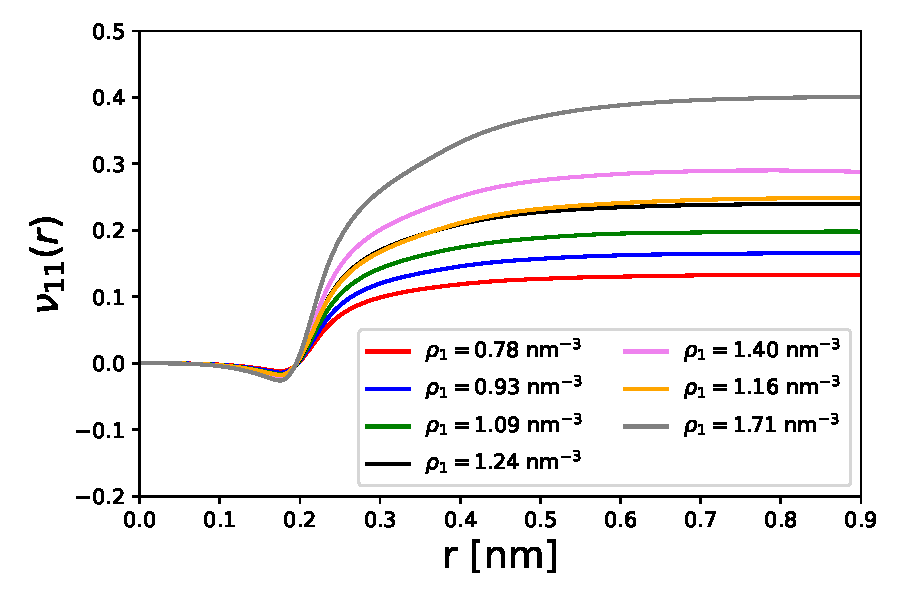
\includegraphics[width=0.5\textwidth]{fig4a.pdf} \\
       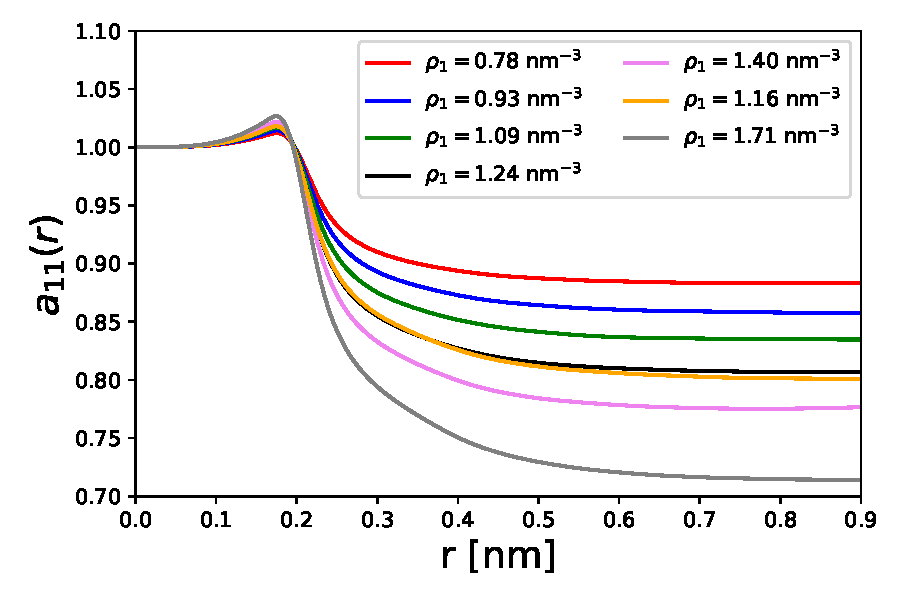
\includegraphics[width=0.5\textwidth]{fig4b.pdf}
        \caption{Top: Running preferential binding coefficient $\nu_{11}(r)$ and derivative of the thermodynamic activity (bottom) for different particle densities in a cubic simulation box of constant length.}
        \label{fig4}
\end{figure}
As can be seen, the converged values are between $a_{11} = 0.7 - 0.9$ which highlights minimal or even moderate differences to the ideal or homogeneous state as denoted by $a_{11} = 1$. Lower values of $a_{11}$ are related to higher particle densities which shows the influence of accumulation effects in comparison to the ideal distribution. One can thus clearly see, that the local structure in terms of surrounding particles strongly affect the derivatives of the thermodynamic acitivity. \\
The corresponding dynamic properties are studied by the mean-square displacement (MSD) for the particles as defined by
\begin{equation}
\label{eq:msd}
\lim_{t\rightarrow \infty} \langle (\textbf{r}_i(t) - \textbf{r}_i(t_0))^2\rangle = 6 D_{11}^st
\end{equation}
with the position $\textbf{r}_i$ of particle $i$ at different times $t$ and $t_0$ and the self-diffusion coefficient $D_{11}^s$. The efficient evaluation of the corresponding values over long particle trajectories can be achieved by the methods outlined  in Ref.~\citenum{maginn19a}. 
All results for the MSDs with regard to different particle densities are shown in the top panel of Fig.~\ref{fig5}. 
\begin{figure}
        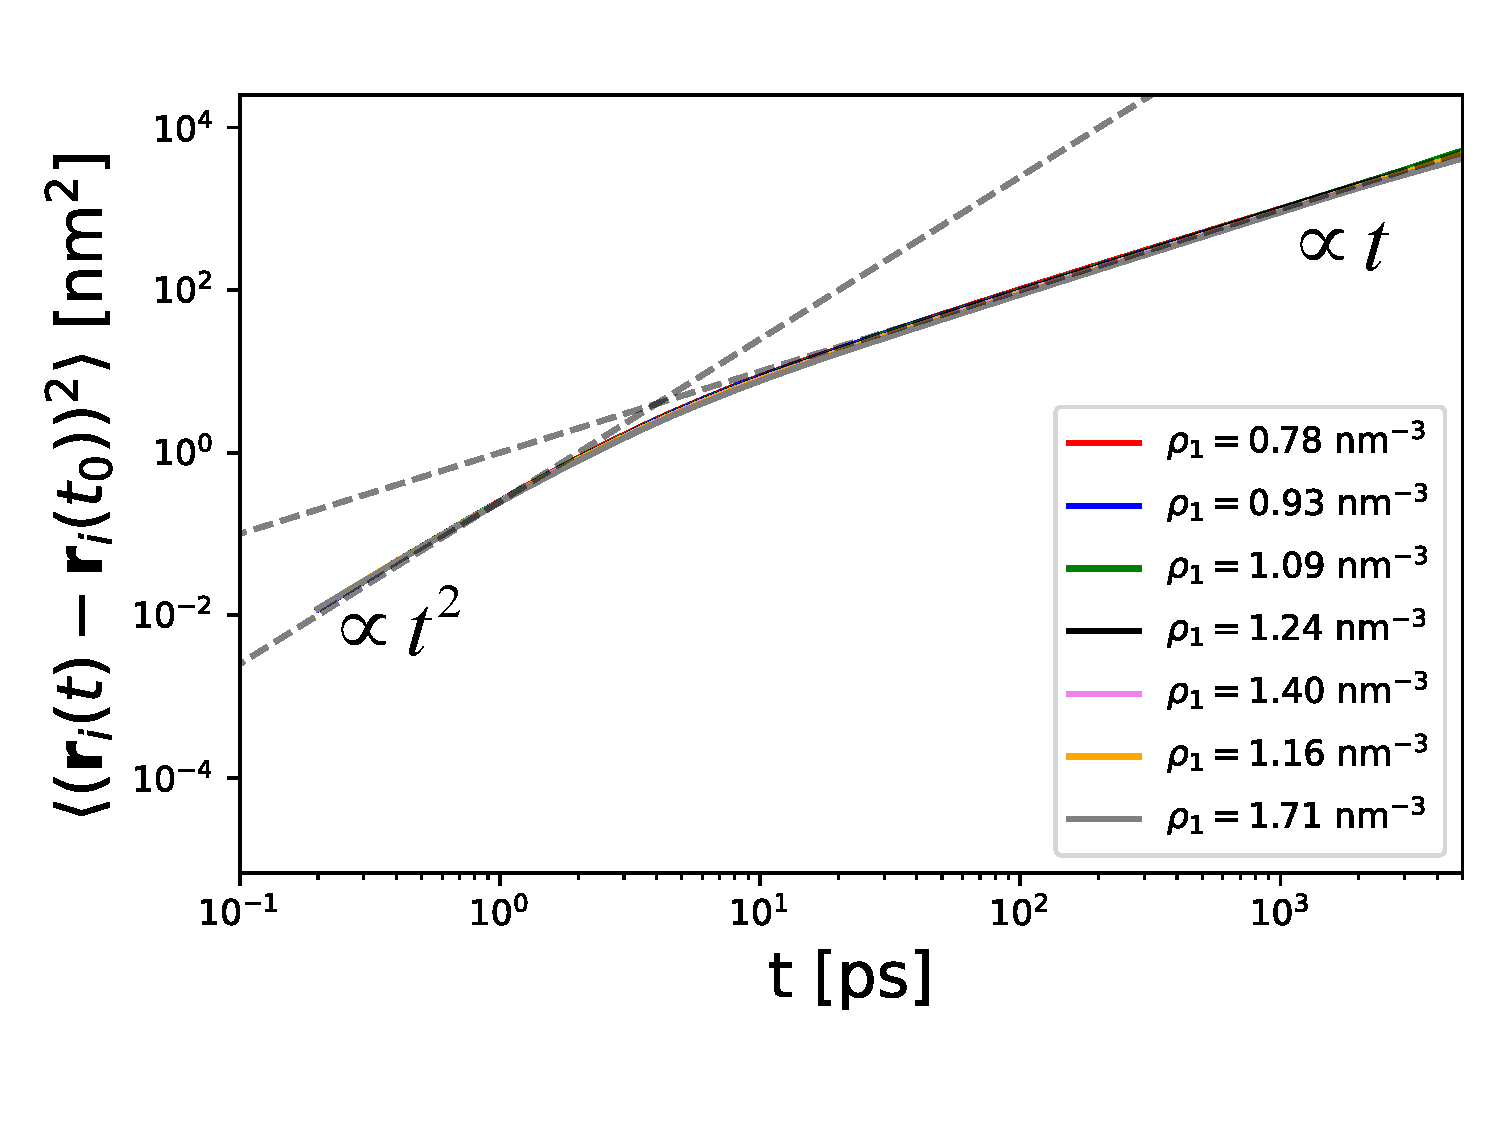
\includegraphics[width=0.5\textwidth]{fig5a.pdf} \\
        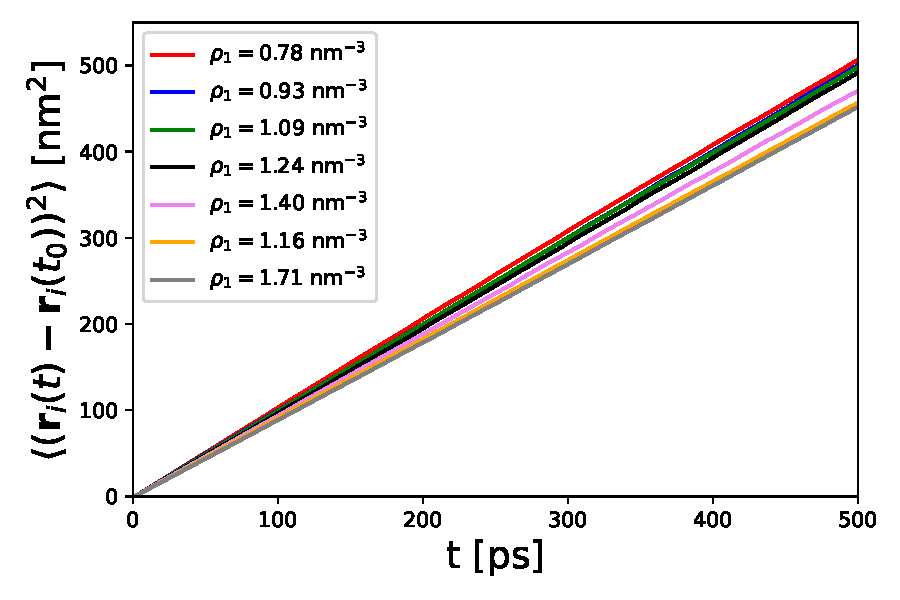
\includegraphics[width=0.5\textwidth]{fig5b.pdf} \\
        \caption{Mean square displacement of particles at different densities in a log-log plot (top) and in linear representation (bottom)..}
        \label{fig5}
\end{figure}
The corresponding representation in a log-log plot (top panel) shows the presence of two regimes which are known as ballistic and diffusive regime \cite{smiatek09a,paul99a}. The ballistic regime scales with $\langle (\textbf{r}_i(t) - \textbf{r}_i(t_0))^2\rangle \propto t^2$ which can be attributed to the initial motion of particles $\langle (\textbf{r}_i(t) - \textbf{r}_i(t_0))^2\rangle \propto v_i^2(t)t^2$ for short times. This finding is also important for Langevin Dynamics simulations (Eqn.~\eqref{eq:LD}), as the mass is not neglected in contrast to Brownian Dynamics simulations. For later times, the particles usually follow the diffusive regime, which is characterized by Eqn.~\eqref{eq:msd} and thus a linear scaling with time $\langle (\textbf{r}_i(t) - \textbf{r}_i(t_0))^2\rangle \propto t$. It can be clearly observed that all particle densities have a comparable transition time between $t = (2 - 10)$ ps, where the diffusive motion dominates. The coincidence of these values shows the non-existent correlations between the particles, so that the transition time depends only on the mass and the friction coefficient.\\
Further evaluation of the MSDs for different particle densities is shown in the bottom panel of Fig.~\ref{fig5}. One can notice that the MSDs significantly decrease for increasing particle densities. For a more detailed study, we considered the MSDs for the time intervals $\Delta \tau = (50 - 100)$ ps to estimate the diffusion coefficients from  Eqn.~\eqref{eq:msd}.\\
The corresponding values for the self-diffusion coefficients $D_{11}^s$ in comparison to the inverse value of $a_{11}(r)$ according to  Eqn.~\eqref{eq:tracerdiff} are presented in Fig.~\ref{fig6}. 
\begin{figure}
        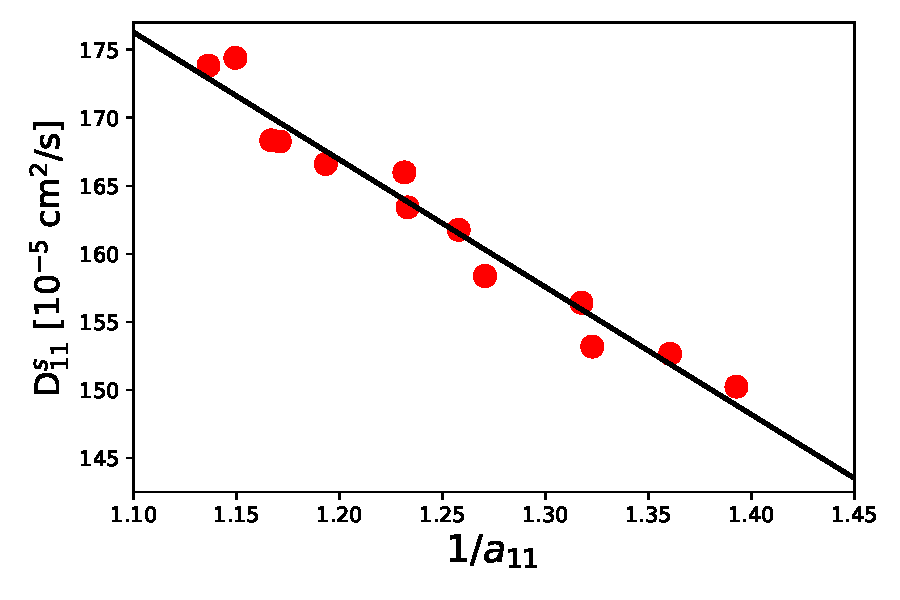
\includegraphics[width=0.5\textwidth]{fig6.pdf} \\
        \caption{Self-diffusion coefficients $D_{11}^s$ for increasing particle densities in comparison to  $1/a_{11}(r)$ (red circles). The corresponding black line shows the results of a linear fit in accordance with Eqn.~\eqref{eq:tracerdiff} with values of fit $D=-16.239\cdot 10^{-5}$ cm$^2$/s and $D_{cm}=188.125 \cdot 10^{-5}$ cm$^2$/s. The correlation coefficient reads $R^2 = -0.99$.}
        \label{fig6}
\end{figure}
The black solid line depicts a linear regression in agreement with Eqn.~\eqref{eq:tracerdiff} with fit values $D=-16.239\cdot 10^{-5}$ cm$^2$/s and $D_{cm}=188.125 \cdot 10^{-5}$ cm$^2$/s. The correlation coefficient reads $R^2 = -0.99$.As can be seen, the corresponding self-diffusion coefficients scale with the inverse of the derivative of the  thermodynamic activity in agreement with Eqn.~\eqref{eq:tracerdiff}. Based on these results, it can be concluded that the local environmentin terms of accumulation effects impacts the self-diffusion coefficients significantly. 

\subsection{Non-Spherical Water Particles}
Corresponding conclusions can also be drawn with regard to non-spherical water molecules as tracer particles in an implicit  continuum solvent. 
The radial distribution functions $g_{11}(r)$ for chosen particle densities  are presented in Fig.~\ref{fig7}. 
\begin{figure}[tbh!]
        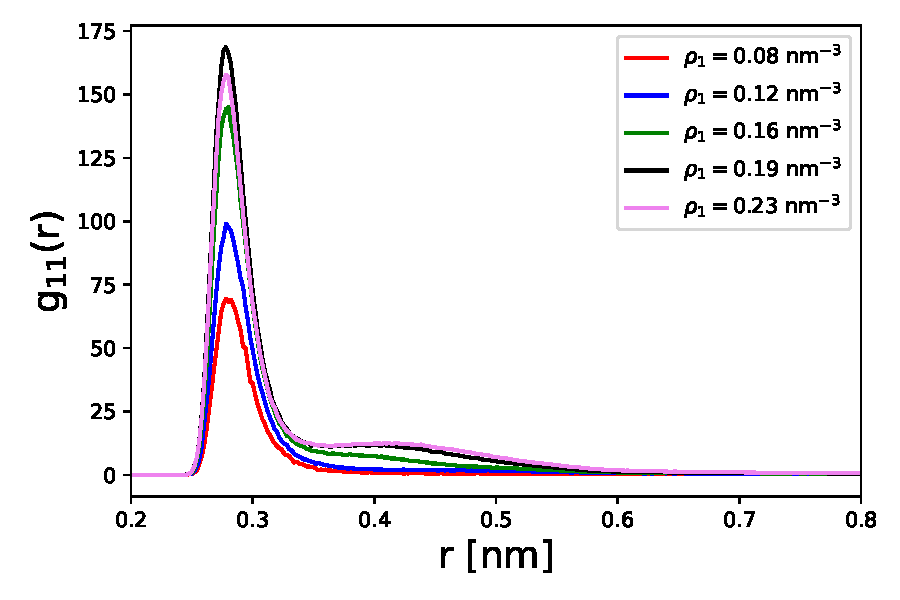
\includegraphics[width=0.5\textwidth]{fig7.pdf} \\
        \caption{Center-of-mass radial distribution functions $g_{11}(r)$ for different water particle densities.}
        \label{fig7}
\end{figure}
In contrast to the results shown in Fig.~\ref{fig1}, the highest particle densities show a reversal in the peak height. Accordingly, the shoulder is more  pronouned for the highest particle density $\rho_1 = 0.23$  nm$^{-3}$ when compared to the second highest density $\rho_1 = 0.19$  nm$^{-3}$. These results can be explained by the non-spherical finite size of the water particles, so that the second contact pair shell is filled when the first contact shell is saturated. However, for all lower densities, an increase of the main peak at $r\approx 0.18$ nm can be observed in good agreement with the previous results.
\begin{figure}[tbh!]
        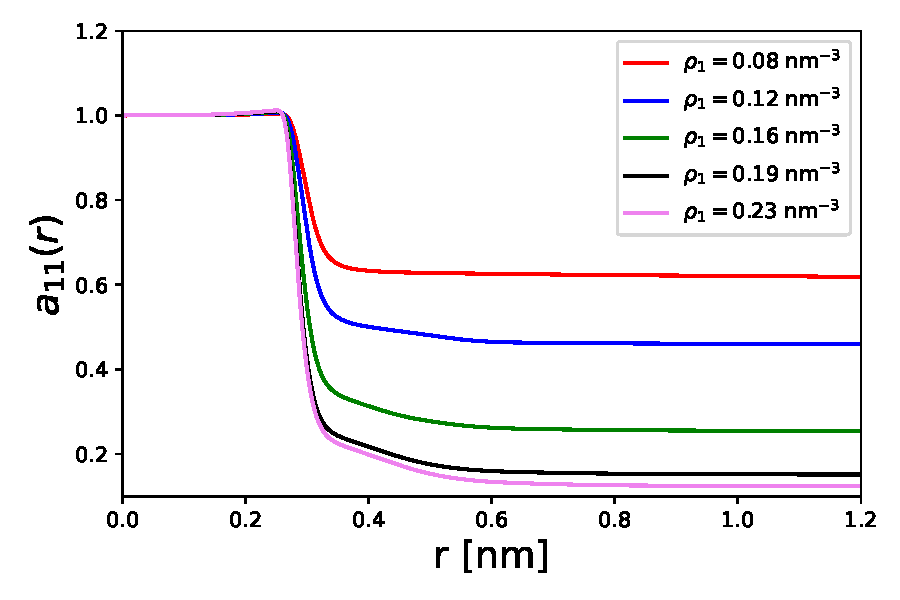
\includegraphics[width=0.5\textwidth]{fig8.pdf} \\
        \caption{Derivative of the thermodynamic activity for different water particle densities.}
        \label{fig8}
\end{figure}
The corresponding effects on the derivatives for the thermodynamic activity concerning different particle densities are shown in Fig.~\ref{fig8}. One can observe a significant drop in the $a_{11}$ values for increasing densities, which is much more pronounced compared to the results for the spherical particles. From this, it can be clearly concluded that highly non-ideal accumulation effects can be observed for the non-spherical water particles.\\
The corresponding values for the diffusion coefficients and the inverse derivatives of the thermodynamic activity are depicted in Fig.~\ref{fig9}. 
\begin{figure}[tbh!]
        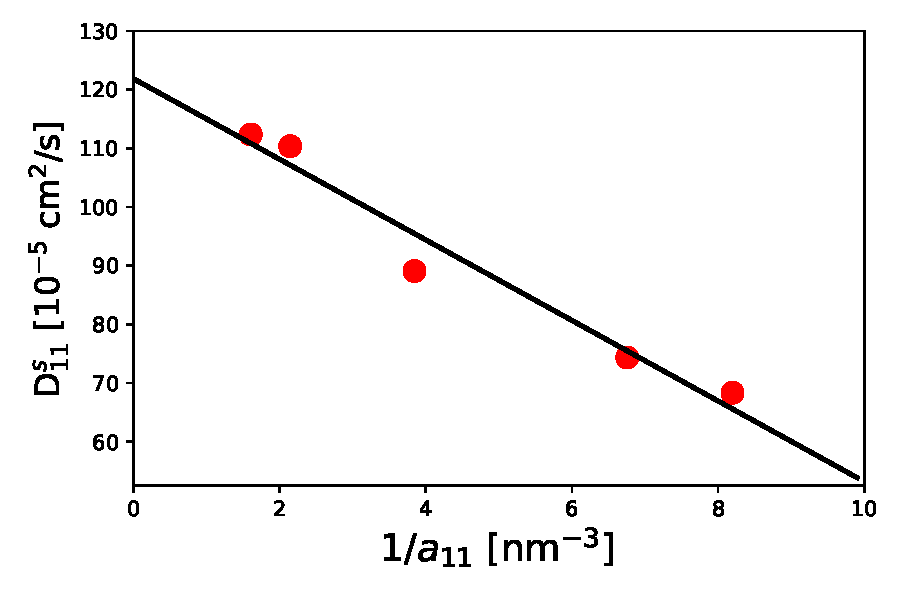
\includegraphics[width=0.5\textwidth]{fig9.pdf} \\
        \caption{Self-diffusion coefficients $D_{11}^s$ for different water particle densities in comparison to  $1/a_{11}(r)$ (red circles). The corresponding black line shows the results of a linear fit in accordance with Eqn.~\eqref{eq:tracerdiff} with values of fit $D=-6.868\cdot 10^{-5}$ cm$^2$/s and $D_{cm}=121.854 \cdot 10^{-5}$ cm$^2$/s. The correlation coefficient reads $R^2 = -0.98$.}
        \label{fig9}
\end{figure}
In agreement with all previous findings, one can also observe a linear relationship which highlights the validity of Eqn.~\eqref{eq:tracerdiff} even for non-spherical particles. A linear fit in accordance with Eqn.~\eqref{eq:tracerdiff} yields $D=-6.868\cdot 10^{-5}$ cm$^2$/s and $D_{cm}=121.854 \cdot 10^{-5}$ cm$^2$/s with a correlation coefficient  of $R^2 = -0.98$.

 

\section{Summary and Conclusion}
We have studied the self-diffusion of spherical and non-spherical tracer particles at different densities in an implicit solvent using LD simulations. In addition, we have also derived an analytical expression for self-diffusion coefficients, based in particular on an interpretation of the thermodynamic factor in the framework of Kirkwood-Buff theory. The results of the simulations are in very good agreement with the analytical expressions, which proves the validity of our considerations. Accordingly, we were able to show that varying particle density is accompanied by a change in the self-diffusion coefficients, which is caused by a change in the derivatives of the thermodynamic activity. However, since the thermodynamic activity is significantly influenced by deviations from the ideal behavior, it can be seen that local accumulation effects and thus the structure of the local environment have a decisive influence on the diffusive properties of the particles. \\
Despite rather low densities and neglected correlation effects in the sense of the Darken equation, it can be clearly stated that the individual molecules influence each other. 
Corresponding accumulation or repulsion effects between the particles can be studied within the framework of Kirkwood-Buff theory \cite{kirkwood51} using Kirkwood-Buff integrals and preferential binding coefficients. As shown in previous publications \cite{ben13a,smith06,smiatek17a}, the derivatives of the thermodynamic activity can be expressed in Kirkwood-Buff integrals for which the complete integration of the corresponding radial distribution functions allows the estimation of the excess volumes. If the particle densities are low and a homogeneous continuum solvent is assumed, which is often the case for stochastic descriptions of particle motion, the corresponding Kirkwood-Buff integrals can be reduced to simple expressions. \\
Accordingly, the derivatives of the thermodynamic activity can be interpreted as an effective mean field, which defines the deviation from the ideality of the distribution in the local environment. If the distribution is ideal, the diffusion coefficients are  not affected. However, if non-homogeneities occur due to accumulation effects, these manifest themselves in a change in the local field, which influences the diffusion coefficients accordingly.  These are not only pure correlation effects, so that the mere presence of other particles can also be of great importance. This reveals an even deeper connection between the individual Fick, Maxwell-Stefan and self-diffusion coefficients, which can all be defined using identical expressions and the corresponding approximations. \\
Our results show that especially the experimental measurement of self-diffusion coefficients can strongly depend on such local environment effects in terms of varying particle densities. It has to be noted that the corresponing results are mainly valid for not only minor deviations from ideality. Hence, one can expect that for very dense solutions further effects may occur \cite{rex08a}. Such lane formation effects in combination with higher order correlation effects as well as hydrodynamic interactions are not considered in our description. Despite these limitations, our findings help to gain even deeper insights into the individual diffusion of particles and to optimize technical applications.

\section{Acknowledgements}
The authors thank Seishi Shimizu, Paul E. Smith and Diddo Diddens for useful suggestions, hints and discussions. 

\section*{References}
\bibliographystyle{aipnum4-1}
\bibliography{ref}
\end{document}
